\section{Introduction}
% context
The web is an invaluable source of data and information about virtually any
subject we can think of. Some of this information is made available to the
public in a semi-structured fashion (e.g., shopping items, news, search engine
results, etc.), providing some level of organization that can be exploited and
leveraged: one can use it to detect/find semi-structured content in a document.
But there are other parts of a document, besides the main content, that can have
some sort of organization (template and menus, for instance), this
``non-content'' organized information adds noise to the extraction process,
decreasing precision. How can we distinguish between them? This is the problem
we tackle in this paper.

% motivation
Extracting structured information, by itself, is an important task, but we must
also be able to identify content, distinguish it from noise, so we do not end up
with an unusable, bloated database, full of unimportant information (i.e.,
noise).
According to \cite{Volume05,TPS2013} between 40\%-50\% of a web document refers
to noise (menus, template, ads), this amount is more than enough to completely
compromise extraction precision.
Since structured data can exist in any kind of web document, whether main
content is structured or not, we must be able to identify it correctly
independently from its source, even when there is no structured content, e.g. we
must be able to identify noise in a textual document as well as in a
semi-structured one.
So, once we have extracted the structured content from a document, how can we
classify it as content or noise? We could not find in literature, nor did we
reach a deterministic and closed form way of doing this, for this reason we
decided to characterize (create hypothesis for the features) content and noise
the best we could and try out machine learning models to approximate a solution.
Our goal is to classify \textbf{structured data}, specifically, as content or
noise, but without restricting ourselves to \textbf{structured content}
documents (i.e., we also want to detect structured noise in textual content
documents). This is a desirable property in order to avoid manual intervention
(selecting only certain types of documents for processing) since the web is
completely heterogeneous in all aspects.

% related work
Previous attempts at this problem, such as \cite{Densiometric08,Noisy03,
Boilerplate10, vieira2006fast}, were targeted at textual content, their
performance is measured in tasks such as clustering and classification of web
pages, not in terms of records extracted.

% {\textcolor{red}{esta frase anterior está meio esquisita}}
 
It is also not clear whether or not these approaches can
be used with structured content, they might remove part of the content,
believing it is noise, without affecting clustering, but this removal would most
likely impair record extraction.
 
% {\textcolor{red}{estás afirmando uma coisa que vais provar? Pelo menos uma
% justificativa dessa tua "crença" deve ser dada, afinal, estás criticando
% trabalhos relacionados e isso não pode ser gratuitamente}}

 Other attempts (\cite{TPS2013,Velloso:2017:ERW:3132847.3132875}), targeted at
structured content, can not be used in an open environment (i.e., one where we
encounter any kind of content: textual, structured  or hybrid), they assume only
structured content will be processed. Although this is not completely
unrealistic it is also not general, demanding more controlled environments of
execution (i.e., more manual intervention needed).

% {\textcolor{red}{este parágrafo está trazendo a discussão de não
% estruturado, semi-est. e estruturado. Mas isso deve aparecer antes, lá no
% parágrafo da motivação... até aqui, não está claro o que tu vais
% consideradar... o título fala em "detectar conteúdo estruturado", mas a tua
% fonte vai ser como? não estruturado, semi-est. e estruturado? não está
% claro}%}

% {\textcolor{red}{os desafios de resolver o problema não vão ser
% discutidos?"How can we distinguish between noise and useful content?" Alguém
% pode achar que é fácil :-) convença-os de que não é :-)}%}

% {\textcolor{red}{eu acho que é necessário uma motivação para o uso destas
% técnicas de ML... da mesma forma que aquele revisor (do email que te mandei)
% comentou, alguém pode dizer que "estão simplesmente testando um monte de
% técnica de ML em cima de um problema"... "qual é o tcham do negócio?"}%}

% proposed approach
In this paper, we analyze several possible supervised machine learning models
for structured content detection. Our investigation considered five machine
learning techniques (Naive Bayes, Support Vector Machine, k Nearest Neighbours,
C5.0 and Logistic Regression) and several combinations of features within each
approach to find the one that suited best in each case. For the extraction phase
we choose the method proposed in \cite{Velloso:2017:ERW:3132847.3132875} because
of the good quality of the results, its feasibility in a production environment
(it is unsupervised and computationally efficient compared to other
state-of-the-art approaches) and also because its source code is freely
available for download, allowing reproducibility of results.
% {\textcolor{red}{parecem justificativas meio esquisitas para usar um trabalho
% que foi feito pelos autores, né? :-) "... its source code is freely
% available". Acho que dá para ser mais direto e colocar apenas que as
% justificativas técnicas e fim de papo}}
The features proposed here are produced during the extraction phase, we just
normalize their values, adding no overhead to the pipeline (once we have the
model trained). We have attained 89\% F-Score in a dataset consisting of 266
different HTML documents from various domains. The novelty presented here lies
in the nature of the features. We are using an alternative representation for
the web documents, to the best of our knowledge this representation was first
introduced in \cite{TPC09}, and until now we have not found any content/noise
detection proposal using features derived from this representation. Our
investigation showed these features can be used to solve this problem
effectively. 
%{\textcolor{red}{DOM tree?? como assim, de onde saiu? Não fale em DOM tree na
% introdução, se estás em um nível de abstração maior... aqui, por
% enquanto, é tudo HTML documents}}

% organization
The rest of this paper is organized as follows: in Section \ref{sec:related} we
present a brief review of related works; in Section \ref{sec:prelim} we
reproduce some concepts needed for the understanding of our work; in Section
\ref{sec:content} we describe and illustrate each feature used in solving the
problem of content detection; in Section \ref{sec:exp} we detail and discuss the
experiments conducted; and in Section \ref{sec:con} we present our conclusions.

\section{Related Work}\label{sec:related}

In our research we have encounter quite a few proposals for web page noise
removal, dating as far back as 1999 \cite{kushmerick1999learning}. Most early
works focused in textual content, where main applications were web page
clustering and classification.

In \cite{Densiometric08,Boilerplate10, vieira2006fast, BlockImp07} the main
content of a web page is assumed to be textual, they might be a fit for a web
page with structured content, but that is unlikely and we have no results
published using these techniques for this purpose, as far as we know.

On the other hand, if we assume content is structured
(\cite{TPS2013,Velloso:2017:ERW:3132847.3132875}) we loose generality and became
confined in this setting. An approach biased toward structured content works
great in a controlled environment but can not perform well in an open
environment where we may encounter textual and hybrid content as well, precision
would drop drastically. There is a cost (usually manual intervention and usually
high) associated with maintaining such a well controlled environment.

% colocar mais referencias aqui
We also found many proposals that do not assume content to be structured or
textual (\cite{Noisy03,Jointop07,SiteOriented11,Entropy09}), but each has some
limitation we intend to overcome in our work. In
(\cite{Jointop07,SiteOriented11,Noisy03}) several samples from the same template
are necessary to train the model, and it only works for that particular
template; and in (\cite{Entropy09}) predefined knowledge bases are required.

Much has changed, since this area of research has started, new applications have
arisen, web development culture has changed, among other things. Due to the
web's ever changing nature, any proposal based on too specific assumptions
(content form, predefined knowledge, template specific, static heuristics rules,
etc.) is deemed to rapidly become outdated.

\section{Preliminaries}\label{sec:prelim}
In this section we outline some concepts needed for the understand of our
proposal.

Since we are proposing a way of identifying structured content and noise, we
need to build our work on top of an extraction technique. We chose the approach
reported in \cite{Velloso:2017:ERW:3132847.3132875} for two reasons: i) the
results reported are equivalent to other state-of-the-art approaches and; ii)
the computational complexity is lower, specially when compared to
rendering-based approaches. This extraction technique uses an alternative
representation for the web documents, a \textbf{tag path sequence} (or TPS), and
here we detail this representation.

\begin{definition}\textbf{(Tag Path)} is a string describing the path from the
root node of the DOM tree to every other node in the tree. For example:
``\texttt{html/body/table/tr/td/\#text}''.
\end{definition}

\begin{definition}\textbf{(Tag Path Code -- TPCode)}\label{def:tpc} is a numeric
ascending code assigned to every different tag path string encountered in the
tree, in order of appearance. If a given path has occurred in the past, it is
assigned the same code as before. The paths are built in depth first order.
Figure \ref{fig:tree2seq} shows an example of this definition. Here we refer to
TPCode as ``symbol'' and a set of TPCodes as ``alphabet''.
\end{definition}

\begin{definition}\textbf{(Tag Path Sequence -- TPS)} is a sequence of TPCodes
in the same order as they were built from the DOM tree. Figure
\ref{fig:tree2seq} shows the resulting TPS for an HTML snippet as  well as the
set of TPCode used for that the sequence. In this paper we also refer to TPS as
simply ``sequence''.
\end{definition}

\begin{figure}[h]
  \centering
     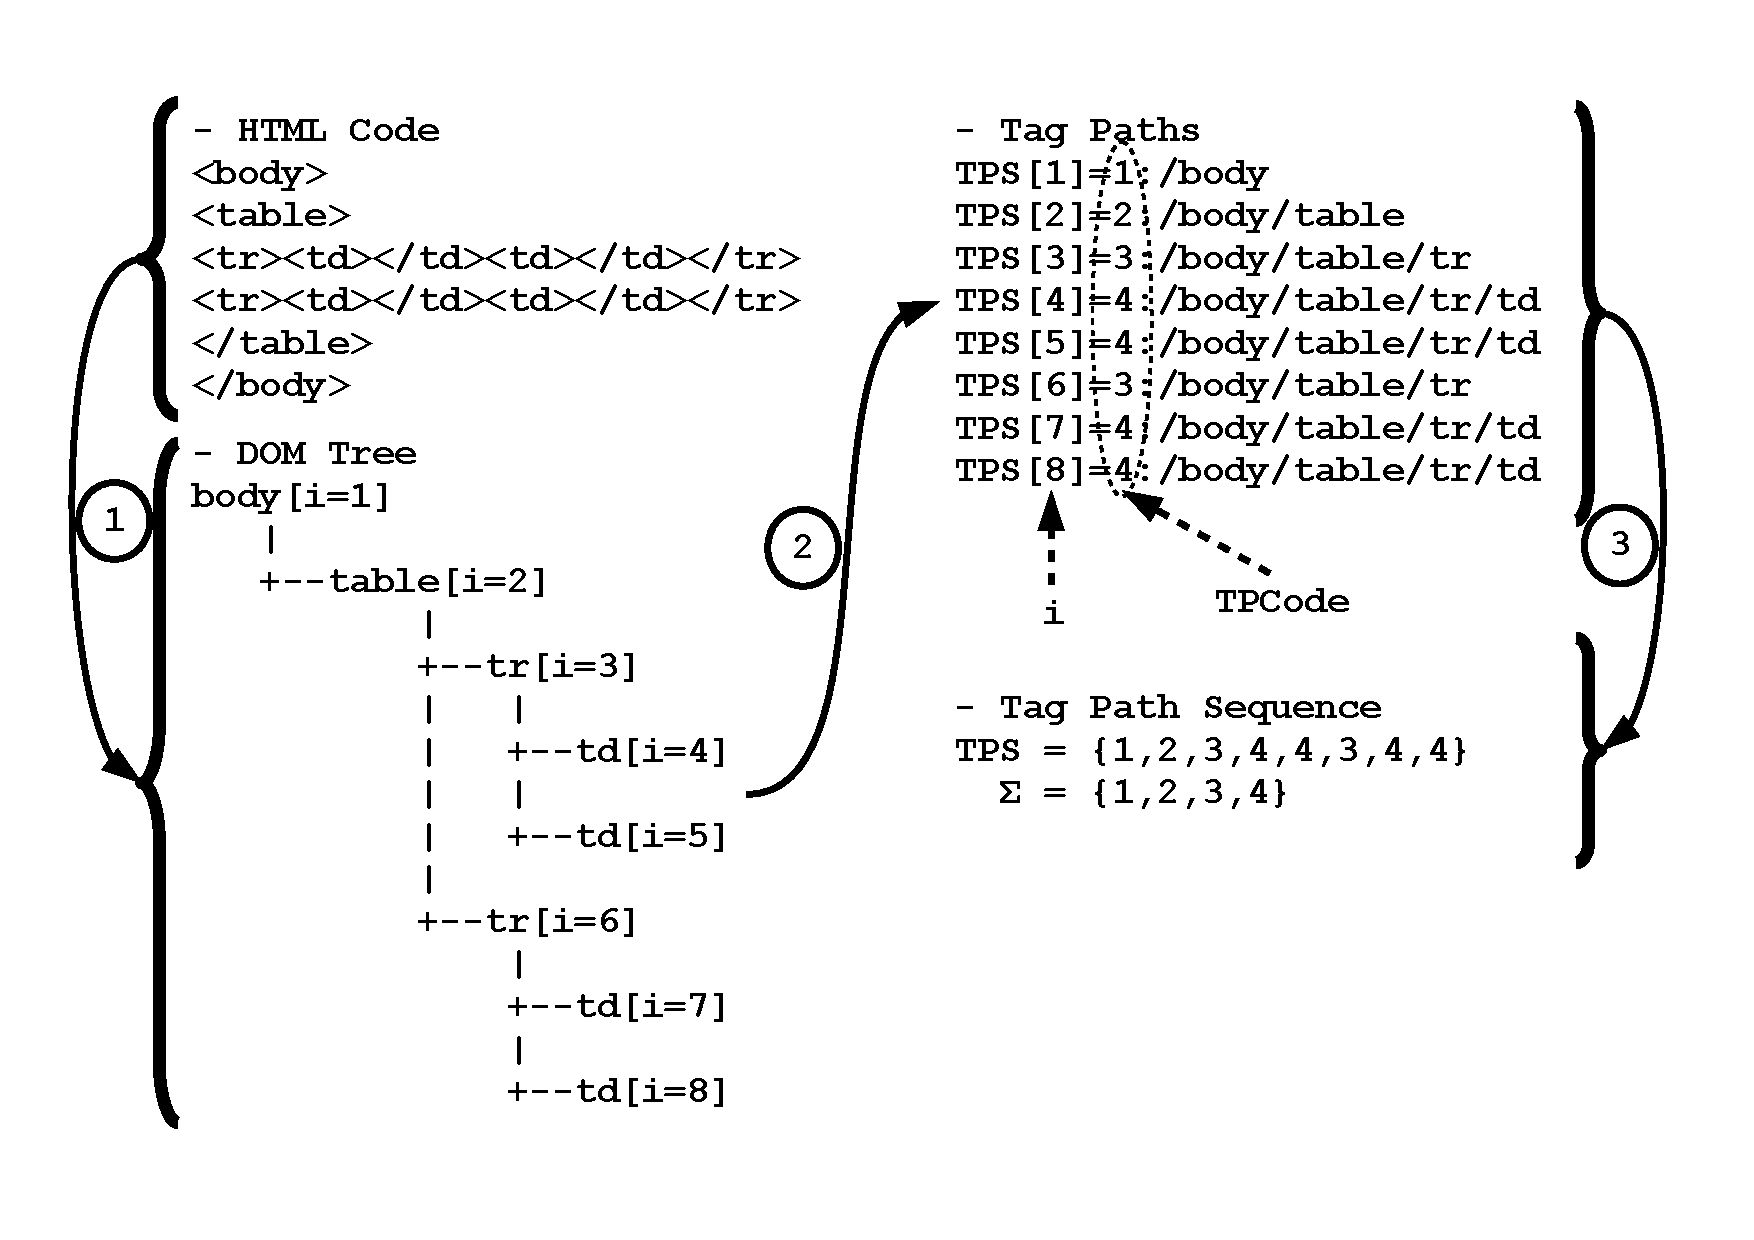
\includegraphics[trim={1.0cm 2.0cm 1.5cm 1.0cm}, clip,  width=\columnwidth]{img/tree2seq.pdf}
  \caption{Conversion of HTML snippet to a tag path sequence.}
  \label{fig:tree2seq}
\end{figure}

\section{Content Regions Detection}\label{sec:content}
In order to distinguish which structured regions are content and which are noise
we consider five region features, such as: size, position, range, record
proportion (count vs size) and angular coefficient (from the region's linear
regression).

These features were chosen because we believe (that is our hypothesis) they
characterize the problem well and thus, can be helpful in solving the problem.
They can also be easily acquired from the extraction technique we are relying
on.

We will discuss each feature in Subsections \ref{ss:size}, \ref{ss:pos},
\ref{ss:range}, \ref{ss:rec}  and \ref{ss:ang} respectively.

\subsection{Size Feature}\label{ss:size}
The region size feature is a real number, between 0 and 1, that represents the
size of the region relative to the entire document, i.e., the percentage of the
document occupied by the region.

The idea behind this feature is that if a web document was designed with the
purpose of depicting a specific content, then this content (the reason the
document was created in the first place) should occupy a considerable portion of
the document. That is, our hypothesis is that the likelihood of a region being
content (and not noise) is directly proportional to its size.

\begin{figure}[h]
  \centering
     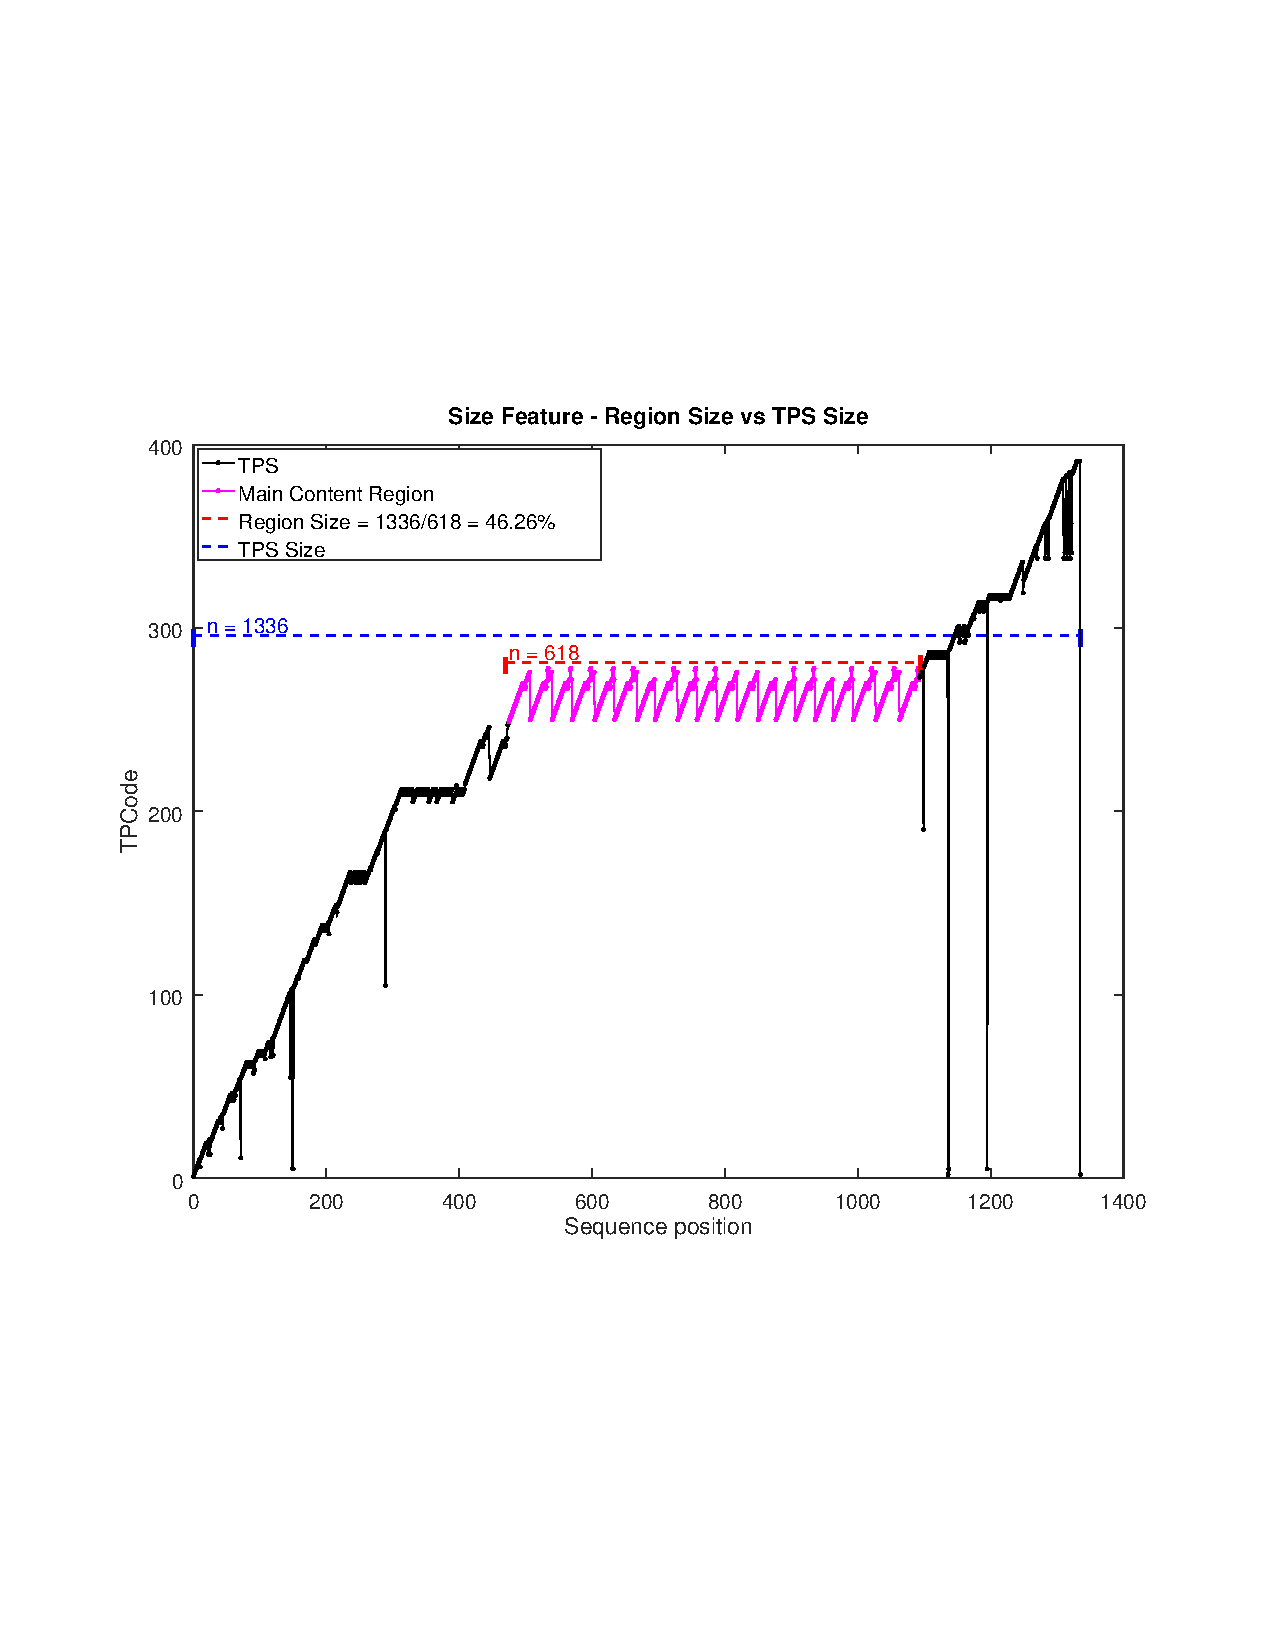
\includegraphics[trim={2.5cm 7.4cm 2.2cm 7.4cm}, clip,  width=\columnwidth]{img/size.pdf}
  \caption{Size feature example.}
  \label{fig:size}
\end{figure}

Figure \ref{fig:size} shows an example where the entire document sequence has
size equal to 1,336 and the main content region subsequence has size 618. The
size feature in this case, using Equation \ref{eq:size}, is equal to
$\frac{618}{1,336} = 0,4625 = 46.25\%$.

\begin{equation}\label{eq:size}
    sizeFeat = \frac{regionSize}{documentSize}
\end{equation}

\subsection{Position Feature}\label{ss:pos}
The region position feature is actually comprised of three position features:
center, horizontal and vertical positions. All three are real numbers between 0
and 1. The \textbf{center position} represents the distance from the center of
the region to the center of the document; the \textbf{horizontal position} is
the distance from the center of the region to the end of the document and; the
\textbf{vertical position} is the distance from the vertical center of the
region to the maximum value of the document.

With respect to the center position, the maximum possible distance is equal to
half document size (e.g, when a region has size one and sits at the start/end of
the document). The value of this feature is a percentage representing how close
a region is from the center of the document (i.e., it is the distance
complement). The rationale of our hypothesis for this feature is similar to the
size feature (Subsection \ref{ss:size}): the closer a region is to the center of the
document, the higher the probability it refers to real content.

\begin{figure}[h]
  \centering
     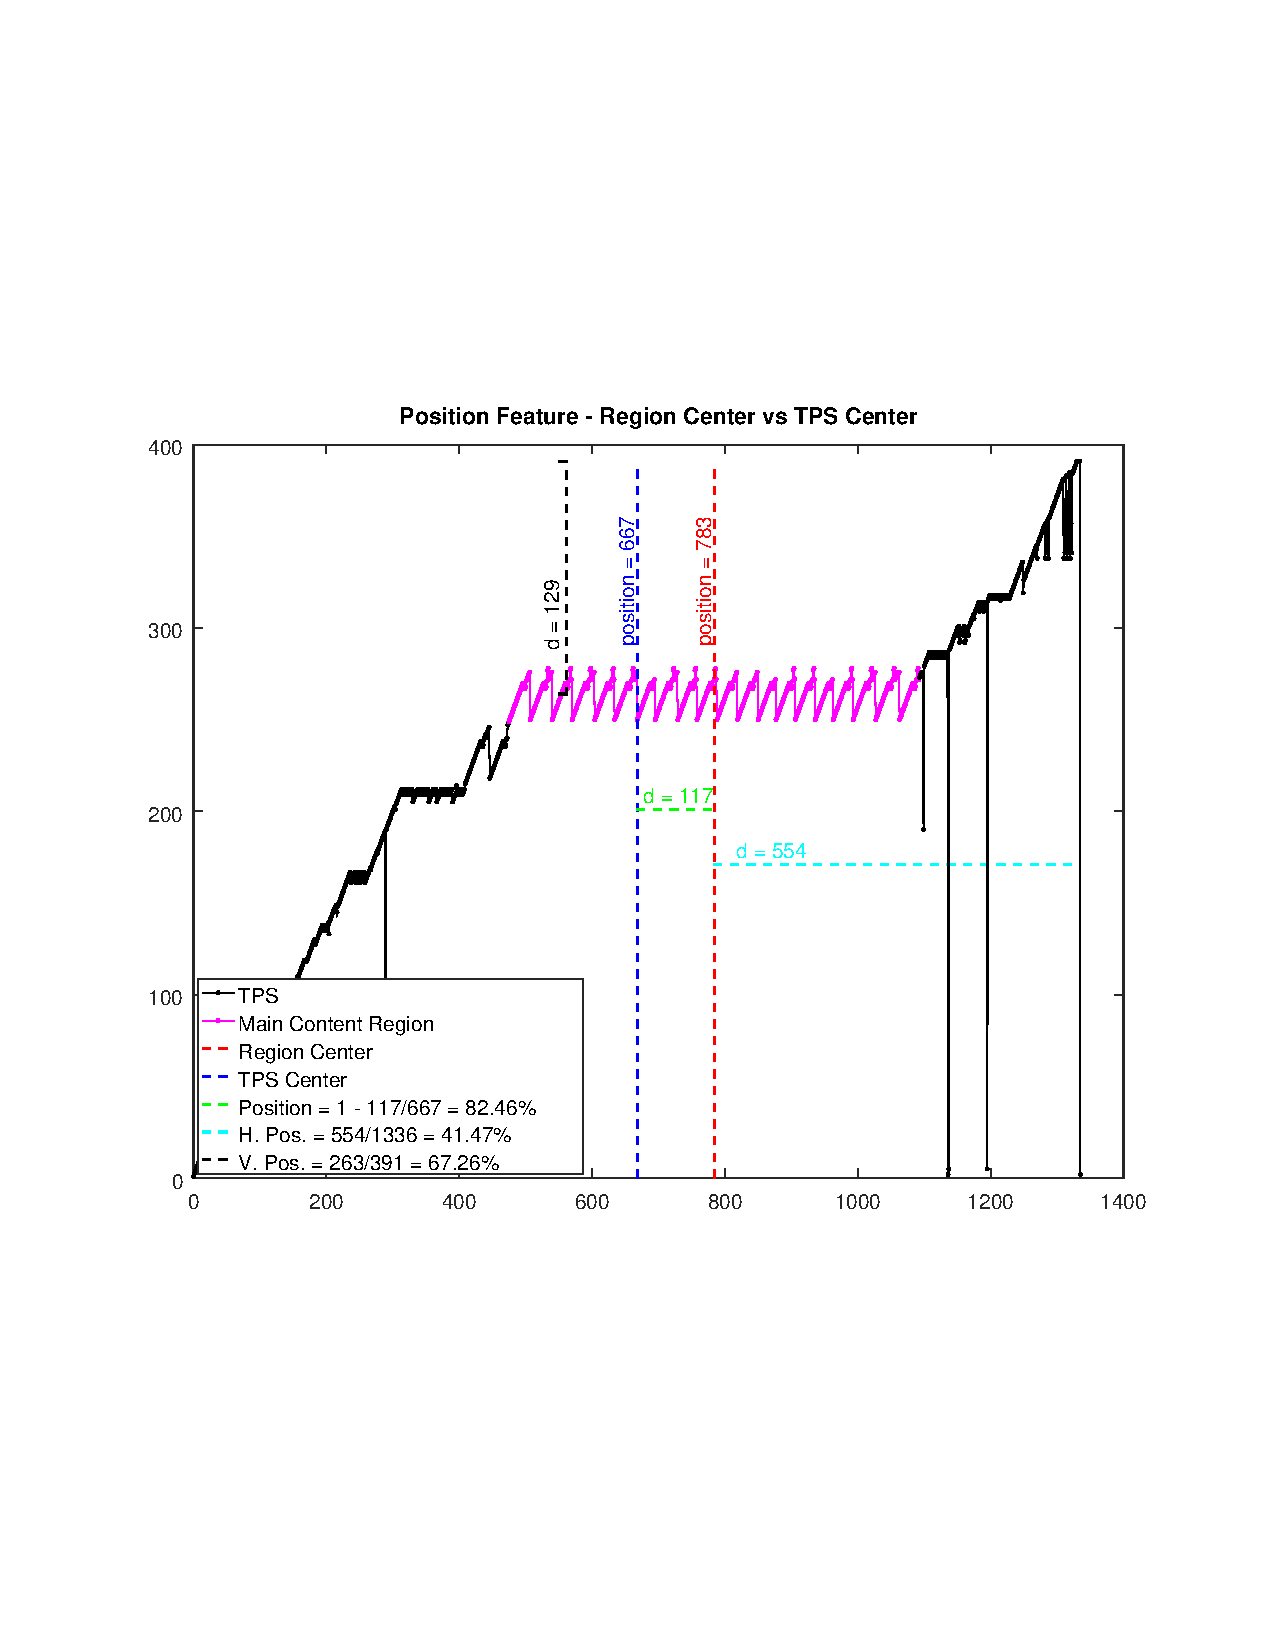
\includegraphics[trim={2.5cm 7.4cm 2.2cm 7.4cm}, clip,  width=\columnwidth]{img/position.pdf}
  \caption{Position feature example.}
  \label{fig:position}
\end{figure}

Figure \ref{fig:position} shows an example where the document center is at
position 667 (this is the maximum distance allowed) and main content region
subsequence center is at position 783, at a distance of 117 from document
center. The value of this feature, using Equation \ref{eq:position}, is equal to
$1- \frac{117}{667} = 82.46\%$

\begin{equation}\label{eq:position}
    positionFeat = 1 - \frac{distance}{documentCenter}
\end{equation}

With respect to the vertical and horizontal position, they are needed to provide
a better indication of a region's position, \textbf{specially} when a document
has no structured content (only structured noise), in this situation a noisy region
will be closer to the extremes of the document, and more distant from its
center. If we were concerned only about documents with structured content, these
two features would, probably, be of little value to us. 

Figure \ref{fig:position} shows how the horizontal and vertical positions are
calculated. The horizontal position is the distance from the center of the
region to the end of the document. Using Equation \ref{}, the value of this
feature igual to $ $. The vertical position is the distance from the horizontal
center of the region (i.e., its average value) to the horizontal end of the
document (i.e., its maximum value). Using Equation \ref{}, the value of this
features is equal to $ $.

\subsection{Range Feature}\label{ss:range}
The range feature is a real number, between 0 and 1, that represents the
percentage of the region range relative to the entire document. It is analogous
to the Size Feature (Subsection \ref{ss:size}) only it is vertical instead of
horizontal. The range is simply the maximum value found in the sequence (or
subsequence) minus the minimum value.

\begin{figure}[h]
  \centering
     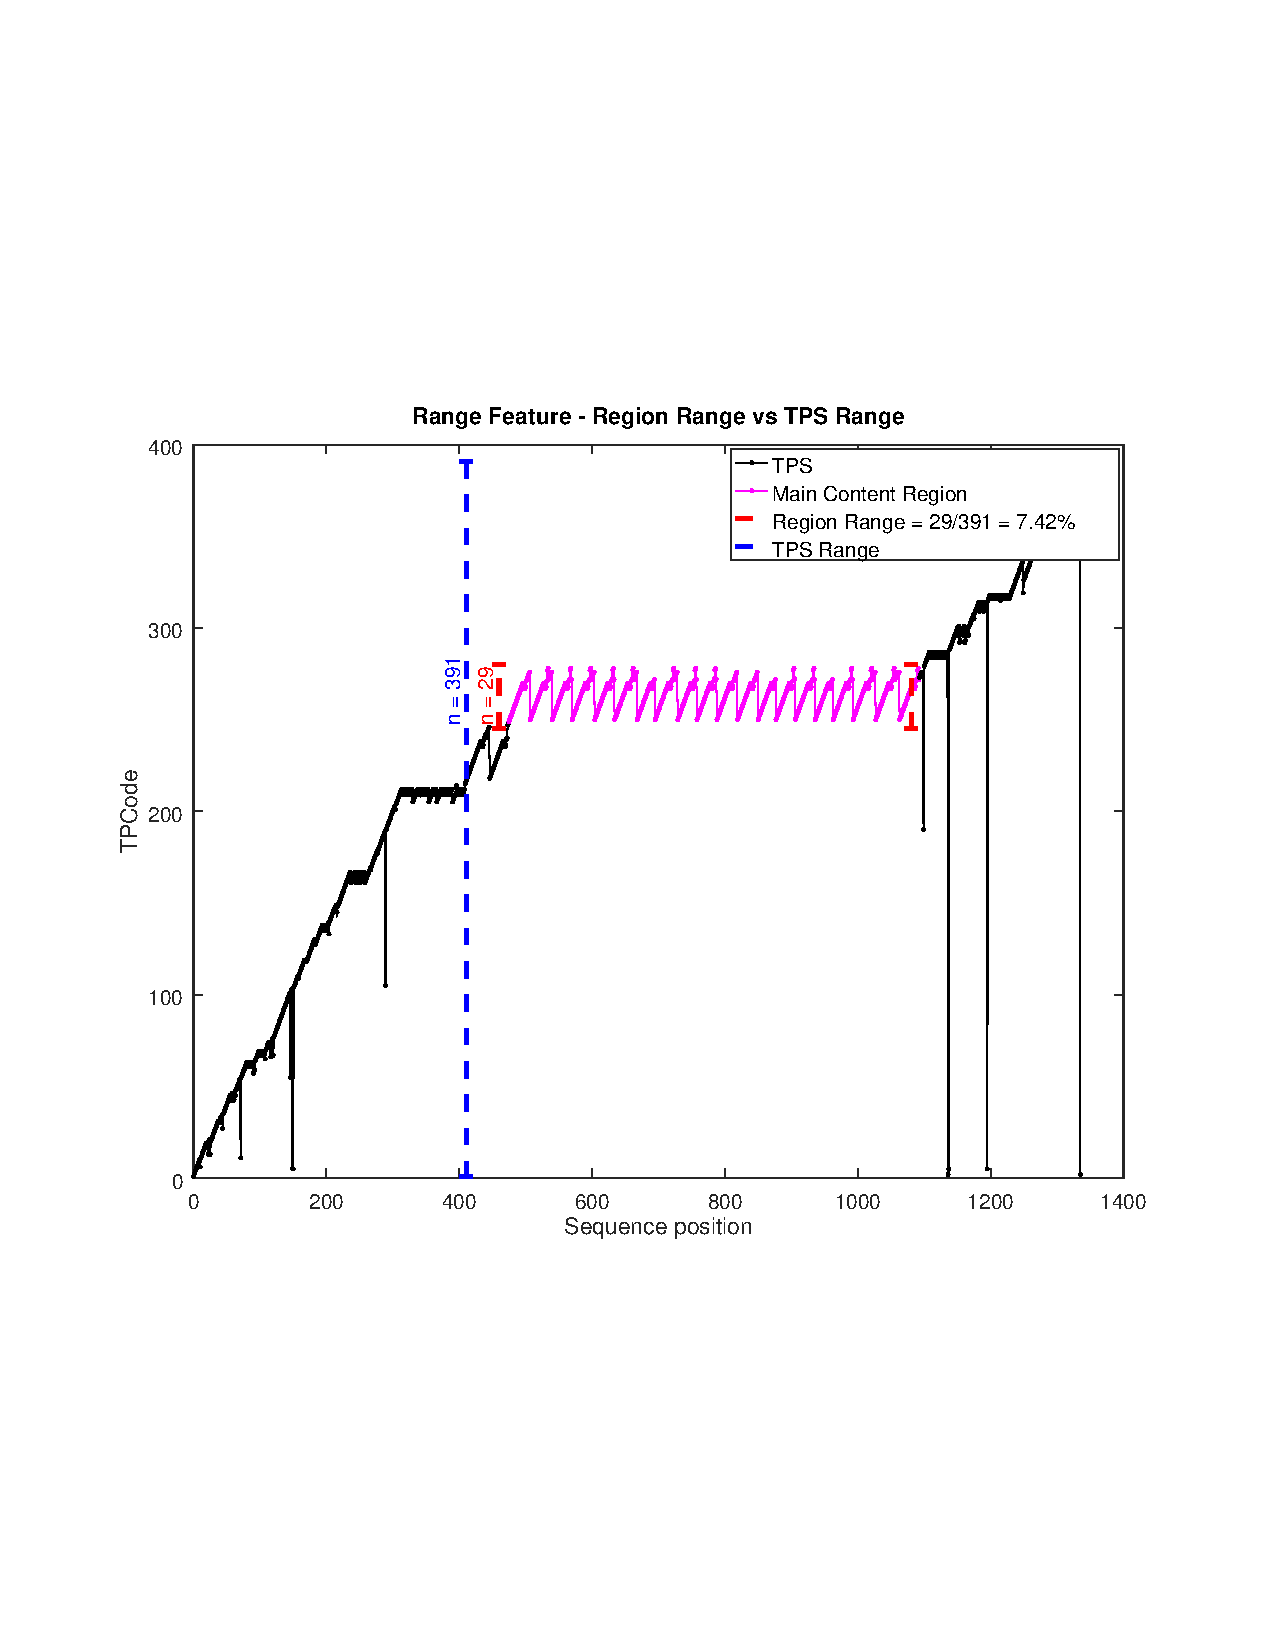
\includegraphics[trim={2.5cm 7.4cm 2.2cm 7.4cm}, clip,  width=\columnwidth]{img/range.pdf}
  \caption{Range feature example.}
  \label{fig:range}
\end{figure}

Figure \ref{fig:range} shows an example where region range is equal to 29 and
document range is equal to 391. The value of this feature, using Equation
\ref{eq:range}, is equal to $\frac{283-254}{391}=\frac{29}{391}=7.42\%$ of
document range.

\begin{equation}\label{eq:range}
    rangeFeat = \frac{regionRange}{documentRange}
\end{equation}

\subsection{Record Feature}\label{ss:rec}
We use the ratio between the number of records and their average size as feature
to indicate if a region is content or noise. We hypothesize that the lack of
proportion\footnote{i.e., a lot of small records or few large records} between
this two measures indicates noise and, conversely, the closer they are from one
another the more likely the region is content. We calculate this value as shown
in Equation \ref{eq:recsize}.

\begin{equation}\label{eq:recsize}
recRatioFeat = \frac{min(numRecs, recCount)}{max(numRecs, recCount)}
\end{equation}

The value of this feature is also a real number between 0 and 1, since the
denominator in Equation \ref{eq:recsize} is always greater or equal to the
numerator.

This two measures are obtained as documented in
\cite{Velloso:2017:ERW:3132847.3132875}, using the region's Fourier transform.
Figure \ref{fig:fft} shows the power spectrum density of the main content region
and its respective record count and average record size. In this example the
number of records detected is 20 and the average size is 31, so the value of the
feature, using Equation \ref{eq:recsize}, is equal do $\frac{20}{31}=64.51\%$

\begin{figure}[h]
  \centering
     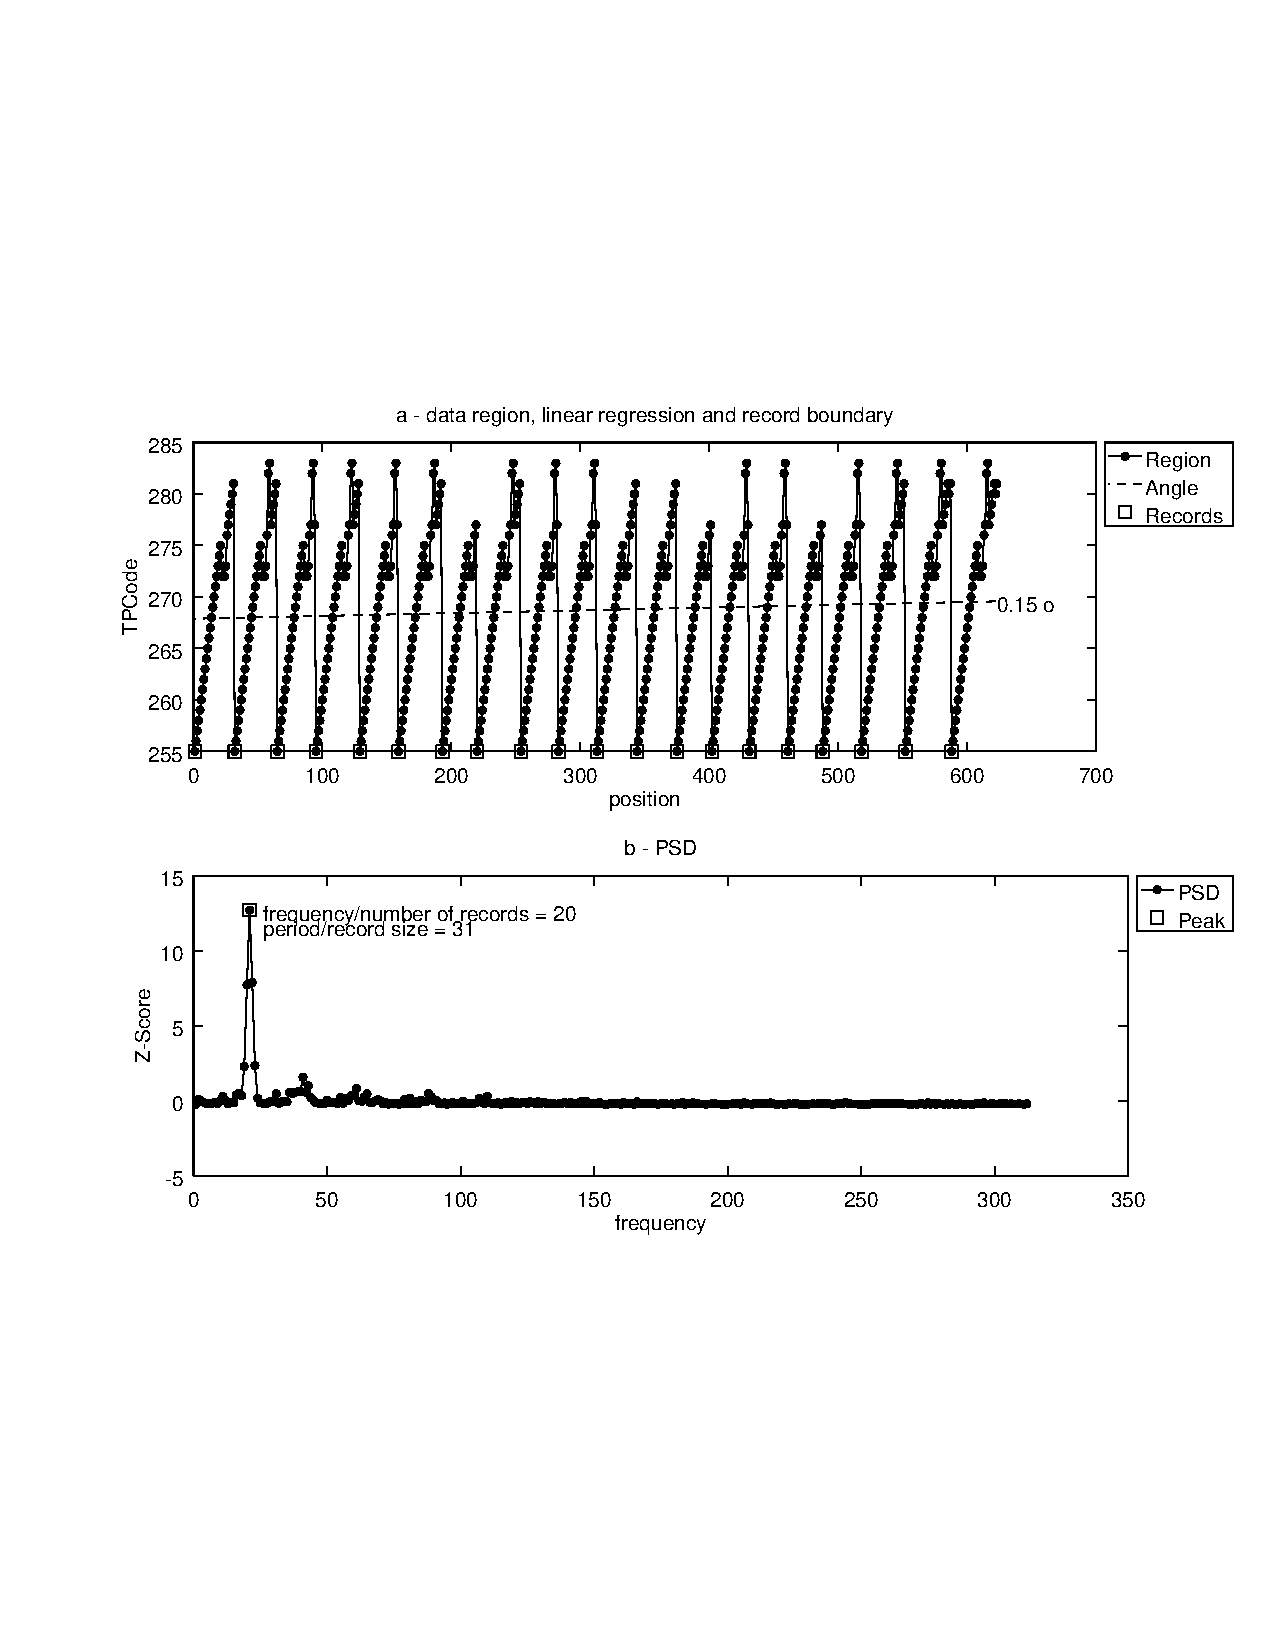
\includegraphics[trim={2.0cm 7.4cm 0.7cm 7.4cm}, clip,  width=\columnwidth]{img/fftreg.pdf}
  \caption{Record count \& size feature example.}
  \label{fig:fft}
\end{figure}

Throughout this paper we will refer to this feature as ``record'' feature.

%\subsection{Angular Coefficient}\label{ss:ang}
%The angular coefficient is used in \cite{Velloso:2017:ERW:3132847.3132875}
%during extraction to detect if a region is structured or not. A low coefficient
%is an indication of structure. We have not constructed an hypothesis around
% this features, we employ it here to investigate if it is also helpful in
%discriminating content from noise.

%Figure \ref{fig:fft} shows the main content region's angular coefficient (0.15
%degrees). We calculate the feature value using Equation \ref{eq:angle}. The
%value of this feature is a real number, between 0 and 1 and it is inversely
%proportional to the region angle since a low angle is an indication of
% structure and the value is relative to the maximum possible angle, which is 45 degrees
%(maximum angle is achieve when there is no structure whatsoever).

%\begin{equation}\label{eq:angle}
%    angleFeat = 1 - \frac{|angularCoeff|}{\frac{\pi}{4}}
%\end{equation}

%Figure \ref{fig:fft} shows an example where the angle is 0.15 degrees. This
%angle corresponds, approximately, to an angular coefficient of 0.0027047, using
%Equation \ref{eq:angle} the feature value is equal to
%$1-\frac{0.0027047}{\frac{\pi}{4}}=99,65\%$

\section{Experiments}\label{sec:exp}

% {\textcolor{red}{em vez de "to achieve the goal of content detection" eu seria
% bem direta e faria um parágrafo que apresente, em uma frase, o(s) objetivo(s)
% dos experimentos (cujos resultados serão apresentados pelas metricas de
% avaliacao com numero plotados nos gráficos)}%}

In this section we detail the experiments we have conducted using supervised
machine learning techniques using the features from Section \ref{sec:content}.
The objectives of this experiments are to determine the subset of features which
are important in this classification problem and measure the classification
performance in terms of precision, recall and f-score.
We have considered, in our study, the following machine learning techniques:
gaussian naive Bayes (GNB), logistic regression (LR), k Nearest Neighbours
(kNN), C5.0 decision trees/rules and Support Vector Machine (SVM).

We have conducted experiments to determine the best combination of features,
within each approach, for solving the problem of distinguishing noise from
content. The procedure employed is to measure the performance using various
combinations of features, starting with each feature separately, to determine
which are key to the problem and which do not contributed to the solution.

For these experiments we have used a dataset consisting of 266 HTML documents
with structured content from various domains (news, banking, hotels, car rental,
tickets, electronics), we use only one page per site to avoid introducing bias
towards specific sites and/or templates\footnote{this is possible because the
extraction approach used also works with a single page input}. These documents
were processed using the technique proposed in
\cite{Velloso:2017:ERW:3132847.3132875}, resulting in a total of 458 regions
that were manually labeled as content or noise (menus, ads, template, etc). This
is the input dataset used for training and validation (randomly partitioned
50\%/50\% in each run) and it is summarized in Table \ref{tab:dataset}. Figure
\ref{fig:dataset} shows a scatter plot of each feature, separately, with respect
to the target class (content vs noise), it gives a rough idea of how content and
noise are intertwined. Table \ref{tab:stat} shows mean and CV for all features
with respect to the target class.

Table \ref{tab:featcorr} shows the correlation between all features. We see that
``size'' vs ``position'', ``size'' vs ``range'' and ``position'' vs ``range''
have a stronger correlation compared to others. Due to that fact we have
investigated how these features behave together in our experiments and found
that no combination of those (in pairs) yielded significant improvements in
f-score, although they usually perform slightly better when combined.

% \textcolor{red}{as legendas das figuras estao iguais... além disso, eu
% colocaria a legenda de noise e content mais visivel (está escondida, eu
% demorei para achar ...:) ) }
 
\begin{table}[h]
\centering
\caption{Input dataset summary.}
\label{tab:dataset}
\begin{tabular}{ | l | l | r |}
\hline
\# Content Regions & 254 & 47.65 \\
\# Noise Regions & 279 & 52.35 \\
\hline
Total & 533 & 100.00 \\
\hline
\end{tabular}
\end{table}

\begin{table}[h]
\centering
\caption{Correlation between all features.}
\label{tab:featcorr}
\begin{tabular}{ | l | l | l | l | l | l |}
\hline
& Size & Record & Range & Vert. Pos. & Hor. Pos. \\ \hline
\multicolumn{6}{|l|}{Content \& Noise} \\
\hline
Position & 0.63 & 0.08 & 0.45 & -0.11 & 0.01 \\
Size & & 0.08 & 0.68 & -0.02 & 0.11 \\
Record & & & 0.08 & 0.04 & 0.03 \\
Range & & & & -0.01 & 0.08 \\
Vert. Pos & & & & & 0.85 \\
\hline
\multicolumn{6}{|l|}{Content} \\
\hline
Position & 0.58 & -0.11 & 0.21 & -0.37 & -0.07 \\
Size & & -0.10 & 0.53 & -0.12 & 0.12 \\
Record & & & -0.04 & 0.04 & -0.04 \\
Range & & & & -0.03 & 0.08 \\
Vert. Pos & & & & & 0.65 \\
\hline
\multicolumn{6}{|l|}{Noise} \\
\hline
Position & 0.25 & -0.01 & 0.22 & -0.15 & -0.11 \\
Size & & -0.12 & 0.39 & -0.15 & -0.11 \\
Record & & & -0.08 & 0.01 & 0.01 \\
Range & & & & -0.13 & -0.09 \\
Vert. Pos & & & & & 0.89 \\
\hline
\end{tabular}
\end{table}

\begin{table}[h]
\centering
\caption{Feature statistics.}
\label{tab:stat}
\begin{tabular}{ | l | l | l | l | l |}
\hline
Feature & Mean & CV & Skewness & Kurtosis \\
\hline
\multicolumn{5}{|l|}{Content \& Noise} \\
\hline
Position & 0.57 & 0.51 & -0.18 & 1.71 \\
Size & 0.27 & 0.87 & 0.92 & 2.90 \\
Record & 0.40 & 0.68 & 0.52 & 2.15 \\
Range & 0.11 & 1.12 & 1.98 & 7.46 \\
Vert. Pos. & 0.55 & 0.47 & -0.26 & 2.14 \\
Hor. Pos. & 0.59 & 0.40 & -0.49 & 2.42 \\
\hline
\multicolumn{5}{|l|}{Content} \\
\hline
Position & 0.74 & 0.27 & -0.81 & 2.95 \\
Size & 0.44 & 0.49 & 0.28 & 2.47 \\
Record & 0.46 & 0.61 & 0.22 & 1.89 \\
Range & 0.19 & 0.74 & 1.49 & 5.51 \\
Vert. Pos. & 0.57 & 0.26 & -0.45 & 3.63 \\
Hor. Pos. & 0.63 & 0.24 & -0.80 & 3.58 \\
\hline
\multicolumn{5}{|l|}{Noise} \\
\hline
Position & 0.41 & 0.65 & 0.58 & 2.16 \\
Size & 0.12 & 0.94 & 2.32 & 9.37 \\
Record & 0.34 & 0.74 & 0.81 & 2.74 \\
Range & 0.05 & 1.40 & 4.37 & 26.83 \\
Vert. Pos. & 0.53 & 0.61 & -0.06 & 1.44 \\
Hor. Pos. & 0.56 & 0.53 & -0.15 & 1.69 \\
\hline
\end{tabular}
\end{table}

\begin{table}[h]
\centering
\caption{Feature Importance (feature vs class).}
\label{tab:importance}
\begin{tabular}{| l | l | l |}
\hline
feature & $\chi^2$ & ANOVA \\
\hline
Size     & 51.6426225  & 487.50116318 \\
Position & 25.8025951  & 260.93679423 \\
Range    & 23.1719961  & 232.44608713 \\
Record   & 4.71168623  & 26.59572956 \\
HPos     & 1.16942710  & 12.38250104 \\
VPos     & 0.433793117 & 3.63505065 \\
\hline
\end{tabular}
\end{table}
         
\begin{figure}[h]
  \centering
     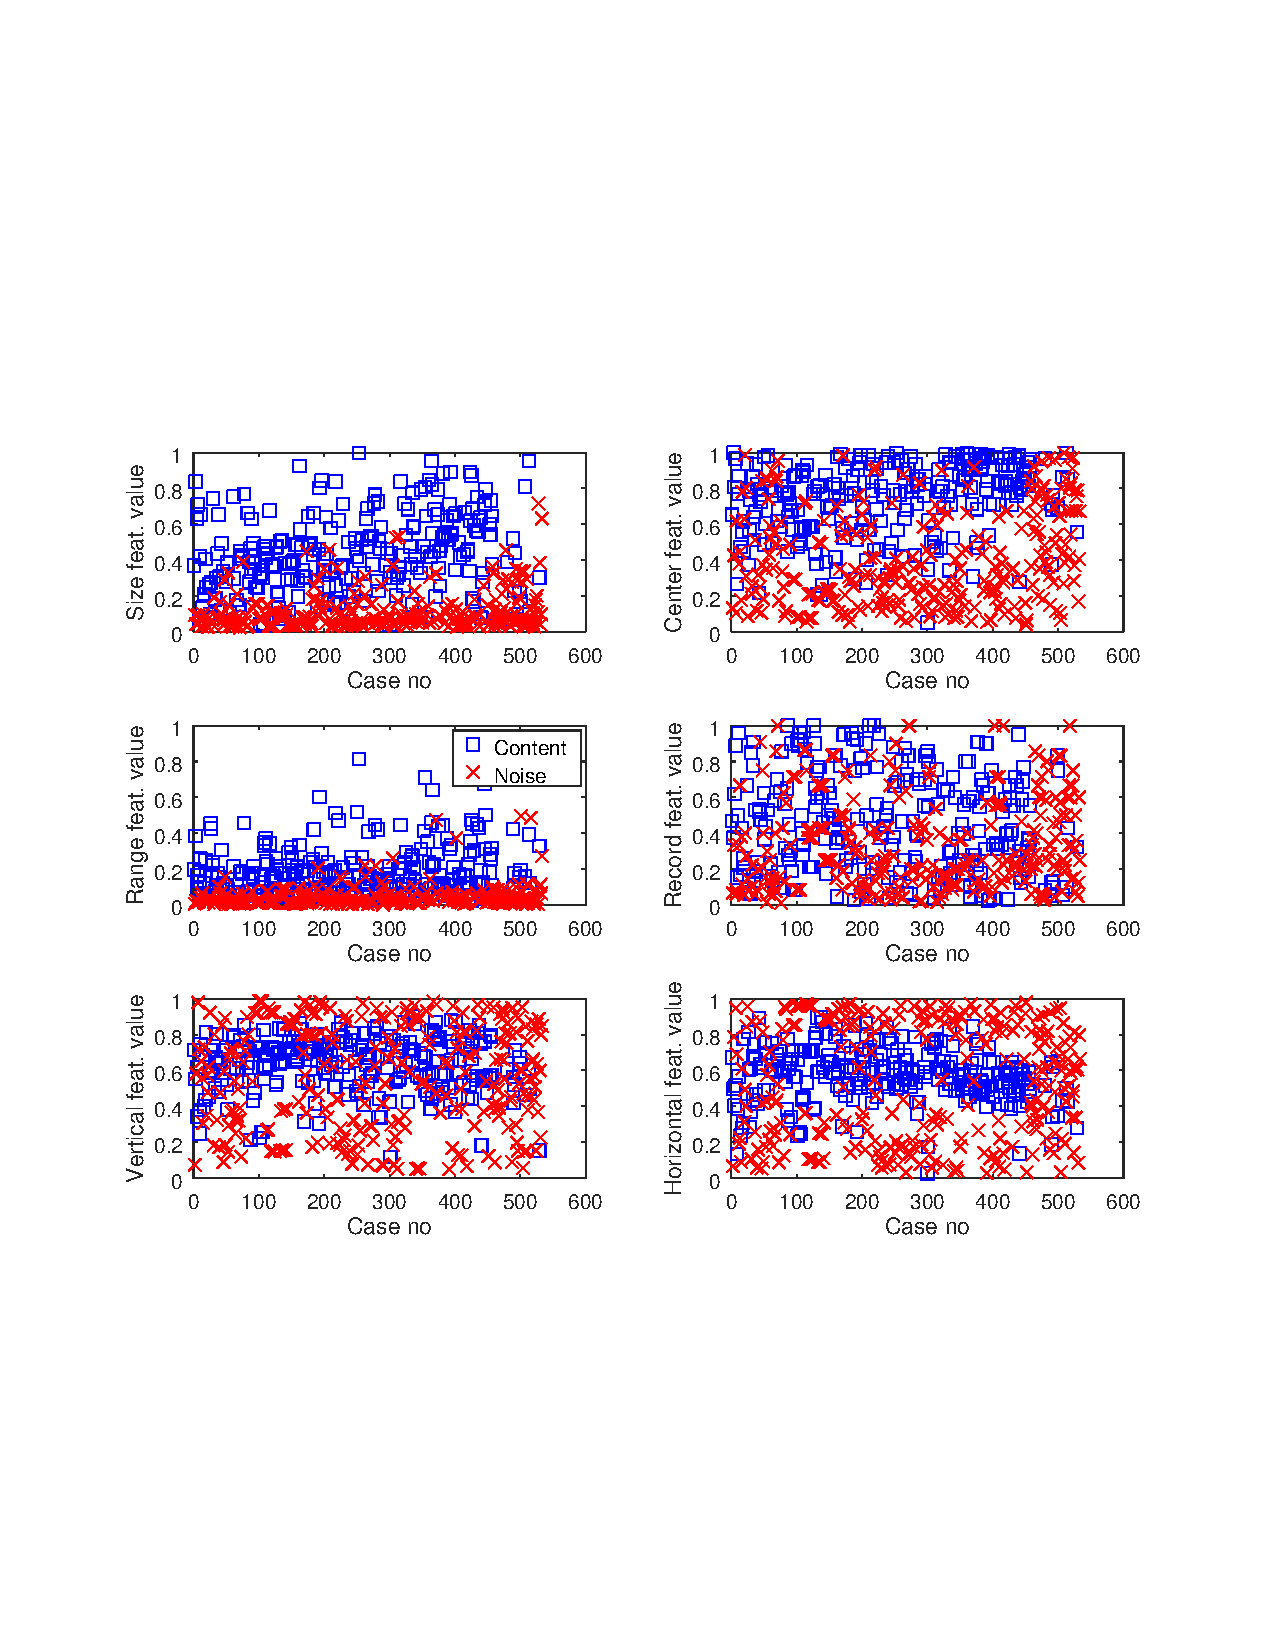
\includegraphics[trim={2.0cm 7.4cm 0.7cm 7.4cm}, clip,  width=\columnwidth]{img/dataset.pdf}
  \caption{Input dataset features: content vs noise.}
  \label{fig:dataset}
\end{figure}

For each approach we've conducted 1,100 random runs/trials from which we remove
the top 50 best results and bottom 50 worst results and reported the average
precision, recall and f-score from the remaining 1,000 runs. At each run we
partition the dataset randomly for training and validation.

In our result tables we are using the following shortening when referring to
feature names: size (\textbf{s}), position (\textbf{p}), range (\textbf{ra}),
record (\textbf{re}) and angle (\textbf{a}). Their combinations is indicated
using the plus signal (\textbf{+}) and the word '\textbf{all}' when all features
are combined.

We detail each experiment, discuss the results and, finally, compare each other.
We will discuss the experiments in Subsections \ref{ss:gnb}, \ref{ss:log},
\ref{ss:c5} and \ref{ss:svm} respectively.

We have adopted the same procedure for all experiments: analyze isolated
features, combine those with best results and add features with worst results,
one by one, to check if they contribute to improve performance. Besides that we
also run experiments combining the highlighted features in Table
\ref{tab:featcorr} (the ones with higher correlation). We have summarized the
results using the standard measures: precision, recall and f-score, plus we also
provide, in the last column, f-score coefficient of variation (CV) to depict the
f-score variability for each feature combination, the lower the CV the better
because it is more likely we can get a result closer to the average out of a
random run of the algorithm.

\begin{verbatim}
MODELPRECRECALLACCF-SCRCV					
LR	90,26%	83,87%	87,60%	86,95%	-4,29%
GNB	81,68%	87,03%	83,64%	84,27%	-5,09%
KNN	87,75%	88,59%	88,35%	88,17%	-1,92%
SVM	86,68%	88,97%	87,77%	87,81%	-3,47%
EXTT	88,31%	88,59%	88,42%	88,45%	-4,05%
XGBC	84,90%	90,54%	87,59%	87,63%	-2,54%
ENSV	88,44%	89,36%	89,09%	88,90%	-3,40%
STCK	88,87%	88,40%	88,76%	88,64%	-3,53%
TPOT	88,60%	88,30%	88,52%	88,45%	-3,13%
------------------------------

MODEL PREC    RECALL  ACC     F-SCR   CV
LR  : 93.23%; 89.33%; 90.61%; 91.24%
GNB : 87.04%; 91.79%; 88.01%; 89.36%
KNN : 90.04%; 90.14%; 89.30%; 90.09%
SVM : 90.41%; 92.17%; 90.61%; 91.28%
EXTT: 92.27%; 92.73%; 91.88%; 92.50%
XGBC: 88.24%; 92.19%; 89.31%; 90.17%
ENSV: 91.20%; 93.42%; 91.70%; 92.30%
STCK: 92.02%; 92.32%; 91.58%; 92.17%
TPOT: 91.54%; 91.62%; 90.91%; 91.58%
\end{verbatim}

\subsection{Gaussian Naive Bayes}\label{ss:gnb}
We start our experiments with Naive Bayes approach. Table
\ref{tab:nbfeatcombres} shows the results for several possible combinations of
features. We can conclude from these results that, using Naive Bayes, the best
feature alone is the ``size'' and the worst is ``record''. We can also see that
not only it is the worst, but it is also counter productive because when
combined with other features it yielded worst results.

The best combination we found, for Naive Bayes approach, is achieved by removing
``record'' from the feature set (f-score 88.31\%). All other features work in
synergy (when we add one of them, we get better results). Although we have
initially hypothesized that should exist some degree of proportionality between
the number of records and their size, that does not seem to true in \textbf{this
case} (using Gaussian Naive Bayes), according to these evidences.

\begin{table}[h]
\centering
\caption{Naive Bayes feature combination results.}
\label{tab:nbfeatcombres}
\begin{tabular}{ | l | l | l | l | l |}
\hline
Features & Precision & Recall & F-score & CV \\
\hline
\multicolumn{5}{|l|}{Combination of features} \\
\hline
s+ra+p   & 0.914715 & 0.840427 & 0.875999 & 0.0171566 \\
s+ra+p+a & 0.911097 & 0.856756 & \textbf{0.883092} & 0.0154882 \\
s+ra+p+re& 0.922310 & 0.735077 & 0.818118 & 0.0460571 \\
all      & 0.921546 & 0.739159 & 0.820337 & 0.0445733 \\
\hline
\multicolumn{5}{|l|}{Single feature} \\
\hline
s        & 0.914287 & 0.818580 & \textbf{0.863791} & 0.0163568 \\
p        & 0.797262 & 0.820565 & 0.808745 & 0.0196024 \\
ra       & 0.923057 & 0.617778 & 0.740176 & 0.0466489 \\
a        & 0.581955 & 0.883760 & 0.701785 & 0.0248184 \\
re       & 0.751081 & 0.132800 & \textcolor{red}{0.225695} & \textcolor{red}{1.7310500} \\
\hline
\multicolumn{5}{|l|}{Pairs of features with high correlation} \\
\hline
s+p      & 0.882599 & 0.856926 & \textbf{0.869573} & 0.0168241 \\
s+ra     & 0.904398 & 0.826890 & 0.863909 & 0.0152281 \\
p+ra     & 0.866504 & 0.822008 & 0.843670 & 0.0177351 \\
\hline
\end{tabular}
\end{table}

\subsection{Logistic Regression}\label{ss:log}
Next we proceed to logistic regression. Again we try several combinations
features, starting with single features and building other combinations on top
of these first results.

Shown in Table \ref{tab:lrfeatcombres}, we see that the best isolated feature
for this approach is ``position'' and worst is ``range''. Although ``record''
performed well alone it showed the highest variability. This approach does not
seem to work well with single features when compared to other approaches adopted
in this paper, probably because this model is not fit for non-linearly separable
data. But when we add other features, increasing dimensions, the results start
to converge with the other approaches.

The best combination we found for logistic regression uses all features (f-score
86.05\%).

\begin{table}[h]
\centering
\caption{Logistic regression feature combination results.}
\label{tab:lrfeatcombres}
\begin{tabular}{ | l | l | l | l | l |}
\hline
Features & Precision & Recall & F-score & CV \\
\hline
\multicolumn{5}{|l|}{Combination of features} \\
\hline
all      & 0.872804 & 0.848496 & \textbf{0.860478} & 0.0178399 \\
p+a+re+s & 0.864550 & 0.837602 & 0.850863 & 0.0184087 \\
p+a+re+ra& 0.835755 & 0.838857 & 0.837303 & 0.0194044 \\
%s+ra+p+a & 0.865408 & 0.808549 & 0.836013 & 0.0180523 \\
%s+ra+p+re& 0.868641 & 0.830611 & 0.849201 & 0.0208313 \\
%s+ra+p   & 0.854419 & 0.780766 & 0.815934 & 0.0189245 \\
p+a+re   & 0.808337 & 0.828931 & 0.818505 & 0.0188616 \\
\hline
\multicolumn{5}{|l|}{Single feature} \\
\hline
s        & 0.977069 & 0.341960 & 0.506613 & 0.0561876 \\
p        & 0.792757 & 0.823705 & \textbf{0.807935} & 0.0190436 \\
ra       & 0.961880 & 0.102638 & \textcolor{red}{0.185483} & 0.1379820 \\
a        & 0.550692 & 0.963034 & 0.700702 & 0.0223186 \\
re       & 0.553701 & 0.923832 & 0.692406 & \textcolor{red}{0.2636230} \\
\hline
\multicolumn{5}{|l|}{Pairs of features with high correlation} \\
\hline
s+p      & 0.865122 & 0.753066 & \textbf{0.805214} & 0.0203305 \\
s+ra     & 0.938936 & 0.657236 & 0.773228 & 0.0331775 \\
p+ra     & 0.823153 & 0.773365 & 0.797483 & 0.0210066 \\
\hline
\end{tabular}
\end{table}

\subsection{kNN}\label{ss:knn}
This algorithm worked better using only the features ``size'' and ``range''
combined (f-score 87.06\%) as shown in Table \ref{tab:knnfeatcombres}. Whenever
we add other features we get worst results with increased variability. kNN also
presented high overall variability, other approaches tended to decrease
variability when more features were added and presented only isolated cases with
higher CV, whereas this one has a higher CV on most feature combinations.

\begin{table}[h]
\centering
\caption{kNN feature combination results.}
\label{tab:knnfeatcombres}
\begin{tabular}{ | l | l | l | l | l |}
\hline
Features & Precision & Recall & F-score & CV \\
\hline
\multicolumn{5}{|l|}{Combination of features} \\
\hline
all      & 0.909575 & 0.785409 & 0.842944 & 0.057421 \\
s+ra+p+a & 0.918977 & 0.765377 & 0.835173 & 0.061300 \\
s+ra+p+re& 0.923357 & 0.758758 & 0.833004 & 0.040087 \\
s+ra+p   & 0.923587 & 0.742281 & 0.823068 & 0.058277 \\
\hline
\multicolumn{5}{|l|}{Single feature} \\
\hline
s  & 0.855220 & 0.842680 & 0.848910 & 0.017819 \\ 
p  & 0.759754 & 0.798229 & 0.778517 & 0.024110 \\
ra & 0.821240 & 0.842640 & 0.831803 & 0.020511 \\
a  & 0.592757 & 0.612325 & 0.602382 & 0.042055 \\
re & 0.621748 & 0.591872 & 0.606442 & 0.046740 \\
\hline
\multicolumn{5}{|l|}{Pairs of features with high correlation} \\
\hline
s+p      & 0.954587 & 0.539115 & 0.689070 & 0.097750 \\
s+ra     & 0.842014 & 0.901301 & \textbf{0.870649} & 0.017291 \\
p+ra     & 0.683811 & 0.960632 & 0.798922 & 0.032261 \\
\hline
\end{tabular}
\end{table}

\subsection{C5.0}\label{ss:c5}

This technique\cite{c5.0} (as well as its preceding versions - ID3\cite{id3} and
C4.5\cite{c4.5}) constructs a decision tree (or a set of rules) selecting first
the features with lower entropy relative to the class/target attribute.
The best combination of features found is ``size'', ``range'', ``position'' and
``record'' (f-score 88.98\%). We can see in Table \ref{tab:c50featcombres} other
combinations with very similar results (e.g., s+ra+p), we believe the reason for
this is that the algorithm has build-in pruning heuristics, eliminating features
that do not contribute significantly, lowering the complexity of the classifier
and improving generalization. Considering this, s+ra+p should be a better pick
than s+ra+p+re.

\begin{table}[h]
\centering
\caption{C5.0 feature combination results.}
\label{tab:c50featcombres}
\begin{tabular}{ | l | l | l | l | l |}
\hline
Features & Precision & Recall & F-score & CV \\
\hline
\multicolumn{5}{|l|}{Combination of features} \\
\hline
all      & 0.884062 & 0.894603 & 0.889301 & 0.0157853  \\
s+ra+p+a & 0.882084 & 0.893372 & 0.887692 & 0.0155015  \\
s+ra+p+re& 0.884565 & 0.895041 & \textbf{0.889772} & 0.0158125  \\
s+ra+p   & 0.884232 & 0.894208 & 0.889192 & 0.0164464  \\
\hline
\multicolumn{5}{|l|}{Single feature} \\
\hline
s        & 0.879768 & 0.874718 & \textbf{0.877236} & 0.0157662  \\
p        & 0.764563 & 0.896252 & 0.825187 & 0.0234265  \\
ra       & 0.808759 & 0.896646 & 0.850438 & 0.0236098  \\
a        & 0.640404 & 0.775778 & 0.701621 & 0.0757501  \\
re       & 0.677834 & 0.568221 & 0.618206 & 0.0670405  \\
\hline
\multicolumn{5}{|l|}{Pairs of features with high correlation} \\
\hline
s+p      &  0.886840 & 0.881957 & 0.884392 & 0.0155634 \\
s+ra     & 0.883394 & 0.885894 & \textbf{0.884642} & 0.0164020 \\
p+ra     & 0.861210 & 0.883945 & 0.872429 & 0.0170438 \\
\hline
\end{tabular}
\end{table}

\subsection{SVM}\label{ss:svm}

\begin{table}[h]
\centering
\caption{SVM feature combination results.}
\label{tab:svmfeatcombres}
\begin{tabular}{ | l | l | l | l | l |}
\hline
Features & Precision & Recall & F-score & CV \\
\hline
\multicolumn{5}{|l|}{Combination of features} \\
\hline
all      & 0.900460 & 0.875131 & 0.887615 & 0.0151347 \\
s+ra+p+a & 0.902895 & 0.872775 & 0.887580 & 0.0148896 \\
s+ra+p+re& 0.907240 & 0.873625 & 0.890115 & 0.0157376 \\
s+ra+p   & 0.905775 & 0.875056 & \textbf{0.890151} & 0.0150039 \\
\hline
\multicolumn{5}{|l|}{Single feature} \\
\hline
s        & 0.900371 & 0.850074 & \textbf{0.874500} & 0.0155069 \\
p        & 0.780726 & 0.874462 & 0.824940 & 0.0191736 \\
ra       & 0.866758 & 0.763723 & 0.811985 & 0.0215323 \\
a        & 0.587373 & 0.853673 & 0.695917 & 0.0243024 \\
re       & 0.529824 & 0.995518 & 0.691582 & 0.0236980 \\
\hline
\multicolumn{5}{|l|}{Pairs of features with high correlation} \\
s+p      & 0.907346 & 0.856814 & \textbf{0.881356} & 0.0144878 \\
s+ra     & 0.900025 & 0.853688 & 0.876244 & 0.0155736 \\
p+ra     & 0.833709 & 0.868877 & 0.850930 & 0.0172262 \\
\hline
\end{tabular}
\end{table}

\subsection{Comparison}
tabela com comparação de todas as abordagens, comentar que são abordagens
supervisionadas vs heuristica não-supervisionada


\begin{table}[h]
\centering
\caption{Results comparison.}
\label{tab:results}
\begin{tabular}{ | l | l | l | l | l | l |}
\hline
& Features & Precision & Recall & F-score & CV \\
\hline
GNB  & s+ra+p+a & \textbf{0.911097} & 0.856756 & 0.883092 & 0.0154882 \\
LR   & all      & 0.872804 & 0.848496 & 0.860478 & 0.0178399 \\
kNN  & s+ra     & 0.842014 & 0.901301 & 0.870649 & 0.017291 \\
C5.0 & s+ra+p+re& 0.884565 & 0.895041 & 0.889772 & 0.0158125 \\
\textbf{SVM} & s+ra+p   & 0.905775 & 0.875056 & \textbf{0.890151} & \textbf{0.0150039} \\
\hline
\end{tabular}
\end{table}

\iffalse
\begin{verbatim}
tech             prec    recall  F1
gauss naiv bayes 98.64\% 57.03\% 72.27\% (very low recall, but highest precision)
LR-SGD           92.11\% 82.03\% 86.78\% (simplest approach, acceptable results)
c5.0             92.80\% 90.62\% 91.70\% (also useful for investigation)
opt k-means      95.06\% 87.83\% 91.30\% (*) has drawbacks/ is biased
svm rbf          95.65\% 85.94\% 90.53\% (equiv do linear, no need to use a kernel)
svm linear       95.69\% 86.72\% 90.98\% (best option, simple with high precision)\end{verbatim}
\fi

\section{Conclusion}\label{sec:con}
